\documentclass[10pt]{article}
%\usepackage[utf8]{inputenc} % Under score not copyable
\usepackage[T1]{fontenc}
\usepackage{geometry}
 \geometry{
 a4paper,
 total={170mm,257mm},
 left=20mm,
 top=20mm,
 }
 
\setlength\parindent{0pt}

\title{Starting with QTcreator}
\author{Valesca Peereboom}
\date{\today}

\usepackage{natbib}
\usepackage{graphicx}
\usepackage{hyperref}
\usepackage{xcolor}

\begin{document}

\maketitle
\noindent This document shows the steps needed to create the FWI project and run the applications and tests in QT creator.

\section{Create FWI project in QT Creator}
Open QT Creator, it automatically starts in the Welcome screen. Create the FWI project by pressing the Open button.
\begin{figure}[h!]
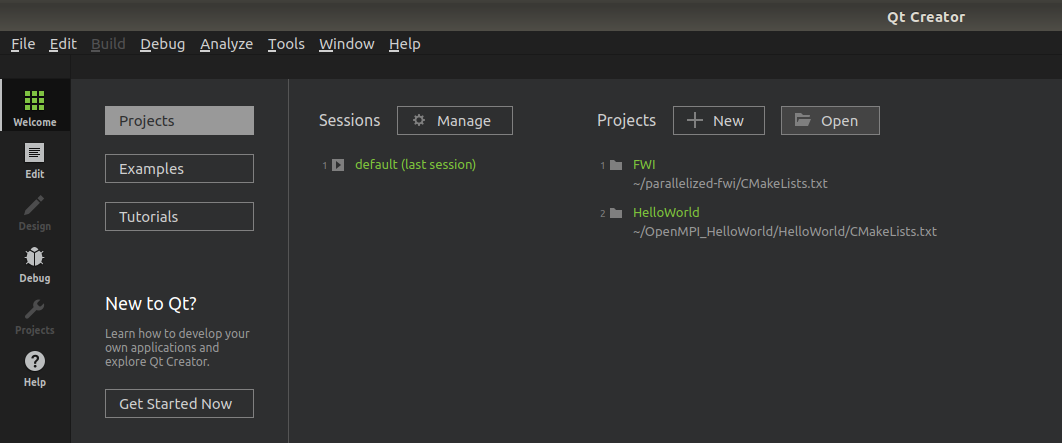
\includegraphics[width = 0.7\textwidth]{DocumentationQT_OpenProject}
\end{figure}

Double click on the parallelized-fwi folder, select CMakeLists.txt and press on Open.
\begin{figure}[h!]
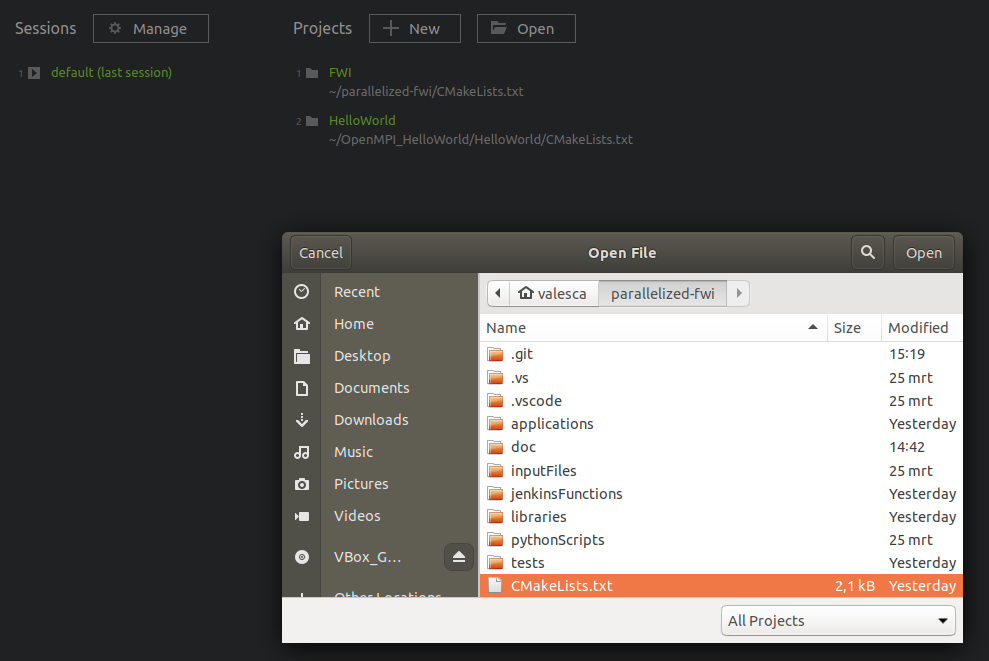
\includegraphics[width = 0.7\textwidth]{DocumentationQT_OpenProject3}
\end{figure}


This automatically should creates the project based on the cmake file.

\section{Run applications}
\subsection{Build}
Go to Projects at the left of the screen. Select in Build \& Run: Build below Imported Kit. At Build Directory: browse to the Build directory.
\begin{figure}[h!]
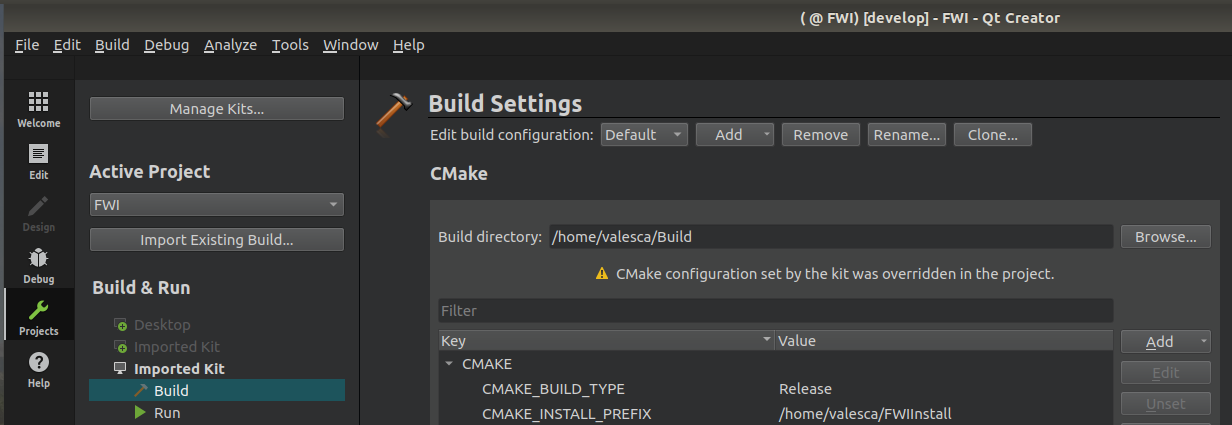
\includegraphics[width = 0.7\textwidth]{DocumentationQT_SetUpBuild}
\end{figure}
Now the project can be build by pressing Ctrl+B or the hammer symbol at the left lower corner.

\begin{figure}[h!]
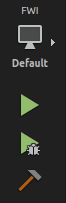
\includegraphics[height = 0.3\textwidth]{DocumentationQT_RunIcons}
\end{figure}

\subsection{Run}
First Copy the default run folder to the home directory by the following commands in the terminal:
\newline
\texttt{ cd \~}
\newline
\texttt{ cp parallelized-fwi/inputFiles/default ..}
\newline

It is important that Preprocess run is executed before a Process can be executed, so make sure that the file \textit{defaultInvertedChiToPressure.txt} exists in the output directory of default. When it does not exists, run the FWI\_Preprocess executable before any other. 
\newline
For this go to Run below Imported Kit at the left side of the screen. Select FWI\_Preprocess in Run configuration in the middle of the screen. Add \texttt{../default} to the command line arguments and choose the Build folder as Working Directory.
The Preprocess can be executed by pressing Ctrl+R or clicking on the green play icon in the left lower corner
\newline

To run the project select the executable in Run configuration, in this case chose FWI\_UnifiedProcess. 
Add to the \textit{command line argument} \texttt{../default conjugateGradientInversion integralForwardModel} and choose the Build folder as Working Directory.

\begin{figure}[h!]
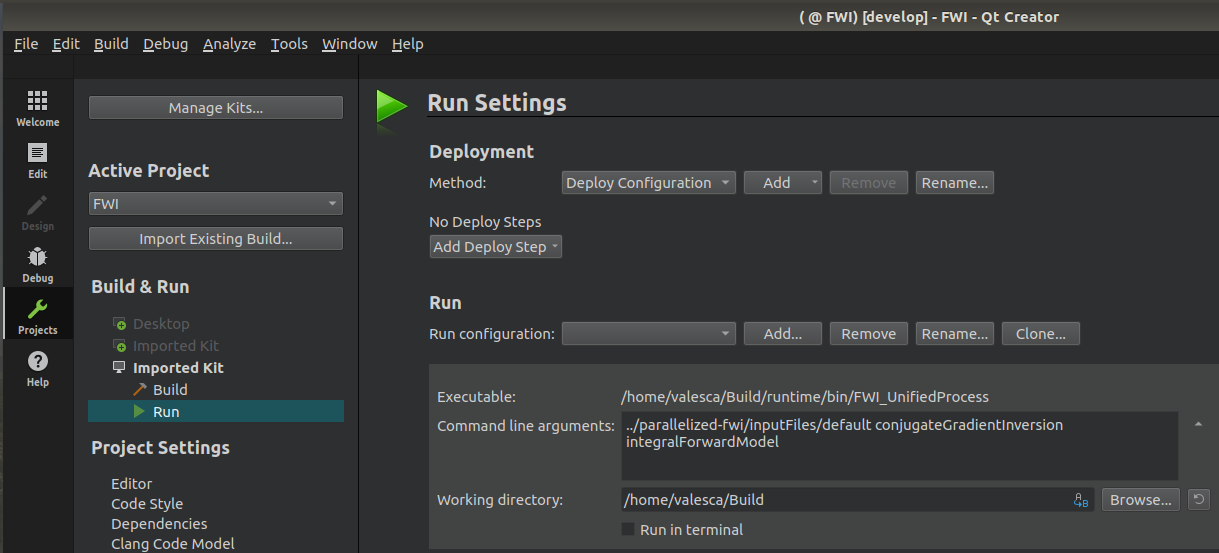
\includegraphics[width = 0.7\textwidth]{DocumentationQT_RunUnifiedProcess}
\end{figure}

The Process can be executed by pressing Ctrl+R or clicking on the green play icon in the left lower corner

\end{document}
